\documentclass[11pt]{article}
\usepackage[utf8]{inputenc}
\usepackage{amsmath, amsthm, amssymb}
\usepackage{graphicx}
\author{Fabian Alenius, Kjell Winblad and Chongyang Sun} \title{Handwritten Character Recgonition}
\begin{document}
\maketitle

\begin{abstract}
Hello.

\end{abstract}

\section{Introduction}
%1. Give general introduction to area.
%2. Describe why it's important.
%3. Applications.
%4. Contributions.

\cite{trec}
%Fabian
testing 123.

\section{Previous work}
%Write about other papers and how they have solved the problem.

\section{Problem}
%Describe our limited version of the problem.
%Describe the two problems, one is recognizing characters and the other is to recognize words.
%1. Images have strokes of width 1.
%2. Assume characters segment in word.

\section{Method}\label{sec:method}
%2. General overview of our implementation.   Kjell
%	Two classifiers
%		What they are doing
%3. Add picture describing implementation.  Kjell

%1. Describe HMM, short overview. Chongyang
%1 Picture of HMM topology
%4. Describe the different initialization algos, advantages and disadvantages. Chongyang
%1.1Topology of HMM Chongyang
%1.2 prevention of underflow. Chongyang
%1.3 Handle zeros in denominator. Chongyang 




\subsection{Dataset}\label{sec:dataset}
%1. Write about creation of sample data. Chongyang
%2. Could not find good dataset. Chongyang
%3. Write down how much data we had. Chongyang
%4. Write about how the word examples are generated

\subsection{Preprocessing}
%1. Write about scaling of picture. Kjell
%2. Segmentation of picture. Kjell

\section{Result}\label{sec:result}
%1. (Started Kjell) Test of different initialization methods and number of training examples for word recognition 
%1. (Started Kjell) Test of different initialization methods and number of training examples for word recognition
%1. Maybe result from character test using different initialization algos.
%2. Basic results from testing the implementation
%3. (Better to do in appendix? Kjell) Depending on how much other results we have, discuss experience of playing around with the gui.

            


\subsection{Word Classifier and Different Initialization Methods}


In this section classification results for the words in table~\ref{tab:words_supported_by_classifier} will be presented. See section~\ref{sec:method}, for a description of the implementation of the classifiers. The training and test example words were randomly generated with the a generator using the properties in table~\ref{tab:word_generator_properties}. See section~\ref{sec:dataset}, for more information about the word example generator. To test the accuracy of the created classifiers, 100 test examples were used. Five test examples for every words. The test examples were generated using the same properties as the training examples. The two initialization methods count based initialization and random initialization were tested with 100, 200, 400, 800 and 1600 training examples. The results of the test is presented in table~\ref{tab:word_classifier_results_generated_data}.

\begin{table}[htb]
  \begin{center}
  \begin{tabular}{ l l l l l }
    dog      & cat       & pig     & love       & hate  \\
    scala    & python    & summer  & winter     & night  \\ 
    daydream & nightmare & animal  & happiness  & sadness \\ 
    tennis   & feminism  & fascism & socialism  & capitalism \\
  \end{tabular}
\end{center}
\caption{Words supported by the resulting classifier.} 
\label{tab:words_supported_by_classifier} 
\end{table}

\begin{table}[htb]
  \begin{center}
  \begin{tabular}{ l l }
    Probability of extra letter at position         & 0.03 \\
    Probability of extra letter missing at position & 0.7 \\ 
    Probability of wrong letter at position         & 0.1 \\ 
    Probability of letter missing at position       & 0.03 \\
  \end{tabular}
\end{center}
\caption{Properties obeyed by the word training example generator.} 
\label{tab:word_generator_properties} 
\end{table}

\begin{table}[htb]
  \begin{center}
  \begin{tabular}{ l l l l l l l }
    NOE    & RIBF   & CBIBT  & RIAT    & CBIAT  & RITT & CBITT \\ \hline
    $100$  & $0.03$ & $0.99$ & $0.01$  & $0.0$  & $6$  & $3$\\ 
    $200$  & $0.02$ & $1.0$  & $0.13$  & $0.36$ & $12$ & $5$\\ 
    $400$  & $0.02$ & $1.0$  & $0.9$   & $0.95$ & $23$ & $7$\\
    $800$  & $0.01$ & $1.0$  & $1.0$   & $1.0$  & $46$ & $13$\\   
    $1600$ & $0.05$ & $1.0$  & $1.0$   & $1.0$  & $96$ & $26$\\  
  \end{tabular}
\end{center}
\caption{Test with different number of training examples and different initialization methods.
	 NOE=''number of training examples for every word'',
         RIBF=''random initialization score before training'',
         CBIBT=''count based initialization score before training'',
         RIAT=''random initialization score after training'',
         CBIAT=''count based initialization score after training'',
         RITT=''random initialization training time (minutes)'',
         CBITT=''count based initialization training time (minutes)''} 
\label{tab:word_classifier_results_generated_data} 
\end{table}

\subsection{Character Classification With Different Parameters}

\begin{table}[htb]
  \begin{center}
  \begin{tabular}{ l | l l l l l l l l l }
    CCF/NOS & 4   & 5    & 6    & 7    & 8    & 9    & 10   & 11 & 12 \\ \hline
    $0.7$  & $30$ & $40$ & $41$ & $37$ & $45$ & $44$ & $48$ & $na$ & $na$\\ 
    $1.0$  & $35$ & $38$ & $39$ & $49$ & $45$ & $44$ & $47$ & $na$ & $na$\\ 
    $1.3$  & $40$ & $45$ & $49$ & $57$ & $57$ & $59$ & $53$ & $na$ & $na$\\
    $1.6$  & $42$ & $49$ & $55$ & $57$ & $56$ & $57$ & $54$ & $na$ & $na$\\   
    $1.9$  & $47$ & $55$ & $52$ & $62$ & $58$ & $59$ & $57$ & $na$ & $na$\\  
    $2.2$  & $50$ & $58$ & $57$ & $65$ & $65$ & $59$ & $62$ & $na$ & $na$\\ 
    $2.5$  & $52$ & $59$ & $61$ & $60$ & $61$ & $63$ & $65$ & $na$ & $na$\\ 
    $2.8$  & $60$ & $60$ & $63$ & $60$ & $60$ & $62$ & $62$ & $na$ & $na$\\ 
    $3.1$  & $na$ & $59$ & $53$ & $64$ & $65$ & $63$ & $65$ & $na$ & $na$\\ 
    $3.4$  & $na$ & $60$ & $62$ & $65$ & $63$ & $67$ & $69$ & $na$ & $na$\\ 
    $3.7$  & $na$ & $63$ & $59$ & $58$ & $63$ & $67$ & $67$ & $na$ & $na$\\ 
  \end{tabular}
\end{center}
\caption{Results for character classification test with different parameters. The scores are percentage of correctly classified characters.
	 NOS=''number of segments'',
         CCF=''component classification factor''}
\label{tab:word_classifier_results_generated_data} 
\end{table}


\section{Discussion}
%1. Discuss the results.
%2. Discuss importance of amount of training data and the effects on performance.
%3. Discuss possibility of training words with data from character classification
%4. Discuss how our approach might work for word recognition

\section{Future Work}
%1. Discuss what other test would be interesting to perform
%2. How can the classifier be improved. More features and real training data for the words?

\bibliographystyle{plain}	% (uses file "plain.bst")
\bibliography{myrefs}		% expects file "myrefs.bib"

\appendix


\section{Source Code}\label{app:source_code}

The source code for the system described in this report can be found at the following Internet location:

\begin{verbatim}
http://github.com/kjellwinblad/HandReco
\end{verbatim}

The source code can be downloaded as a ZIP-archive or cloned using git\footnote{http://git-scm.com/}.

\section{Result Reproduction}\label{app:result_reproduction} 

The test results presented in section~\ref{sec:result} are produced by scripts written in the Jython\footnote{Jython is a version of Python for the Java Virtual Machine (http://www.jython.org/)} programming language. The following steps will run the test scripts:

\begin{enumerate}
 \item Follow the instructions in appendix~\ref{app:source_code} to download the source code for the system.
 \item Follow the instructions in the \verb|README.md| file in the root of the source code directory. These instructions will help you to set up your environment for running the test scripts.
 \item Open a system terminal and execute the following commands (Notice that the path may look different in your system):
 \begin{enumerate}
  \item \verb|cd /path/to/HandReco/src/test|
  \item To run tests for word classifier:
  \item \verb|jython word_classifer_tester.py|
  \item To run tests for character classifier:
  \item \verb|jython character_classifier_tester.py|
 \end{enumerate}
\end{enumerate}

\section{Testing Handwriting Recognition in Graphical User Interface}
%Kjell Describe the GUI for running the HandReco Writer and perhaps some comments on how it works
A graphical user interface (GUI) has been created in order to test the handwriting recognition system in practice. See figure~\ref{fig:hand_reco_writer_screenshot} for a screenshot of the graphical user interface. The following steps can be used to run the GUI:

\begin{enumerate}
 \item Follow the instructions in appendix~\ref{app:result_reproduction} to step 2.
 \item Open a system terminal and execute the following commands (Notice that the path may look different in your system):
 \begin{enumerate}
  \item \verb|cd /path/to/HandReco/src/gui}|
  \item \verb|jython hand_reco_writer.py|
 \end{enumerate}
\end{enumerate}

The GUI can only recognize capital Latin letters. To see which words are available for word corrections click on the \textbf{Info$\Rightarrow$Available Words...} menu item. To input a character, first paint the character in the paint area and then press the \textbf{Write Character} button. To do a space, press the \textbf{Space} button. To do a space and let the word classifier correct the last word, press the \textbf{Space and Correct} button.

    \begin{figure}[htb] 
      \begin{center}
	\leavevmode
	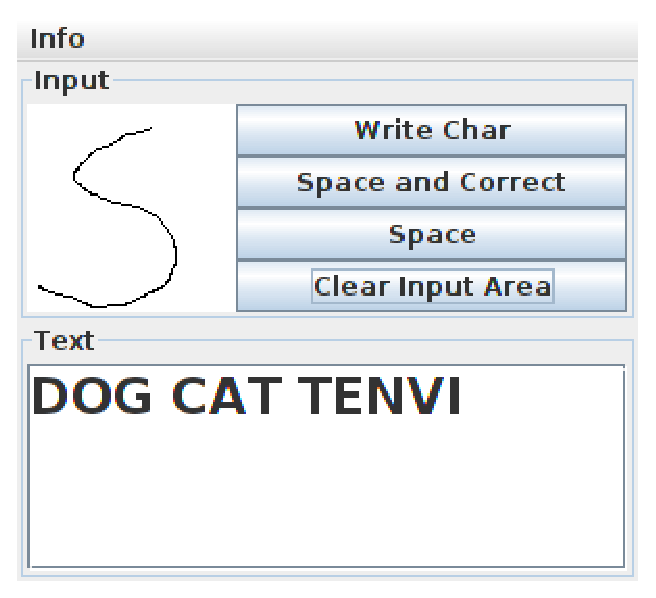
\includegraphics[width=80mm]{Screenshot_HandReco_Writer.eps}%width=115mm,height=40mm
      \end{center}
      \caption{Screenshot of HandReco Writer.}
      \label{fig:hand_reco_writer_screenshot}
    \end{figure}


\end{document}